\chapter{Implementing the Fault Detector}

After all the baseline foundations of deep learning and convolutional
neural networks have been derived, it is now time to apply these
methods to the problem of fault detection in the CLAS12 drift
chamber. Due to the CLAS12 productive environment heavily relying on
the JAVA ecosystem, all implementations are carried out utilizing
the JAVA programming language as well. The basis of the autonomous
fault detection system is formed by the deeplearning4j (DL4J)
library which is briefly described in the following section.

\section{The Deeplearning4j Library}

Deeplearning4j is an open-source deep learning library written for the
JAVA Virtual Machine (JVM). It is supported by the well known
AI-Startup Skymind and contains implementations of many algorithms
from the artificial intelligence domain, such as convolutional neural
networks, that will be used when implementing the fault detector.

To speed up the computations that have to be performed during the
training of deep convolutional architectures, DL4J relies on its own
numerical backend engine, ND4J, that contains C++ and Cuda
implementations of all required operations, most importantly matrix
multiplications. This way, deep neural networks can be trained on
big clusters containing multiple CPUs and GPUs, leveraging the huge
amounts of parallelism introduced by these computational
architectures.

Additionally, the DL4J library also provides useful mechanisms that
make monitoring the training process highly accessible, such as
Web-UIs which offer visual representations of the loss function as
well as the weight updates during training. Evaluating the trained
classifier is also not a difficult task, as DL4J provides
designated classes that are designed to compute all the relevant
metrics on the training dataset.\footnote{See
  \url{www.deeplearning4j.org} for more information.}

\section{Data Preparation}

Before the data can be fed into a convolutional neural network, a few
steps of preparation are necessary. Recall the heatmap plots of
different faults shown in section \ref{sec:faults}. The data that will
be presented to the network will be organized in the form of a \(6
\times 112\) array representing the activation level of each wire in a
superlayer, similar to the heatmaps. This way, the spatial structure
that is present within the data is preserved, which is essential when
working with CNNs, because as shown in section \ref{sec:convnets},
these architectures heavily depend on structural assumptions on the
input. Unlike in the case of images, the fault data will only consist
of a single channel, resulting in an input volume of size \(6
\times 112 \times 1\).

Due to the fact that activation levels can vary drastically among
different regions, regions far away from the electron beam receiving
less particles passing by, the data has to be normalized in order to
compensate for these effects of disproportion. This is done by projecting
the activation values within each input on a numerical scale between 0
and 1, the lowest activation ending up at 0, the highest at 1. This
procedure will make it easier for the network to ignore the
differences in absolute activation levels and focus more on the local
fault patterns instead.

\section{The Fault Detection System}

When looking at the examples of various faults that can occur in the
drift chamber (see section \ref{sec:faults}), it becomes apparent that
there are usually multiple faults happening within a single
superlayer (see for instance Fig. \ref{fig:dead-connector}, where
there are a dead connector as well as multiple dead wires present in
the data). To account for this circumstance, multiple CNNs are
trained on the fault data, each individual CNN only specializing in
recognizing a single fault type (see section \ref{sec:faults} for a
summary of the different fault types), thus
resulting in a binary classifier for each fault. To obtain information
on the various faults present in a single input, each individual CNN
is presented with the corresponding data. In the next step, all the
individual responses are collected, resulting in a list of faults that
were recognized within the given superlayer. The network architecture
used is similar for each CNN that is part of the fault detector as
described in the following section.

\subsection{Network Architecture and Configuration}

After the \(6 \times 112 \times 1\) input volume resulting from the
normalized activations of a superlayer, a convolution layer
is inserted as the first feature extractor of the network. The layer
uses a kernel size of \(2 \times 3\) which accounts for the
unsymmetrical dimensions of the input. The total number of kernels
within this layer, i.e. the amount of features to look for, is set to
20 and a stride of 1 in each direction is used. The ReLU is applied
as an activation function to this layer.
Following the convolution layer, a max-pooling layer is employed with a
filter size of \(1 \times 2\) and a stride of \(1 \times 2\) as
well. This is done in order to compress the feature data along the
``wire''-dimension. After the pooling layer, a single fully
connected hidden layer with 100 hidden neurons is inserted, utilizing
the ReLU activation function as well. The output layer consists of two
output neurons, one firing if the designated fault was detected, the
other firing if not. The softmax activation function is used on this
layer to make the ouputs interpretable as probabilities. An
illustration of the network architecture used in the fault detector
can be seen in Fig. \ref{fig:fault-architecture}.

The weights and biases of the network are initialized using the Xavier
method (see section \ref{sec:xavier}), ensuring a weight distribution
that enhances network trainability. As for the optimization algorithm,
a slight variation of the traditional stochastic gradient
descent algorithm (see section \ref{sec:stochastic}) is employed,
called ADADELTA. The advantage of this algorithm is that it is able to
adjust the learning rate during training based on the local
characteristics of the loss function by scaling the gradients based on
previous updates, resulting in a fairly robust procedure
\cite{adadelta}. The gradients in each step of the updating process
are computed using the backpropagation algorithm (see section
\ref{sec:backpropagation}).

\begin{figure}[h]
  \centering
  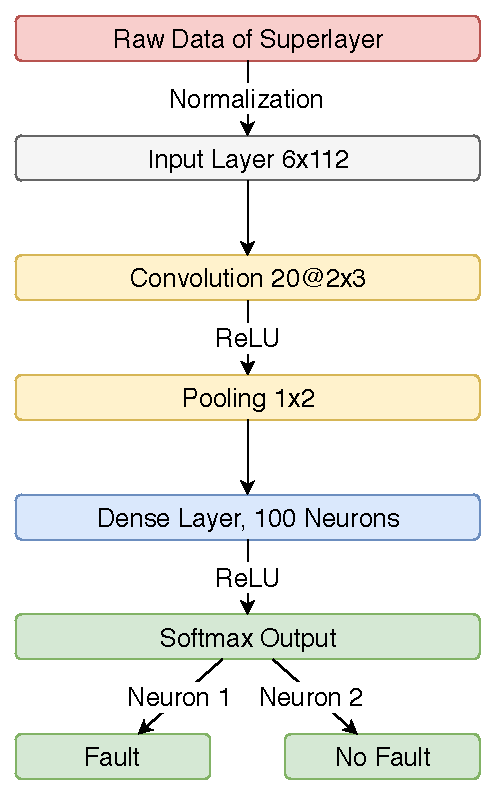
\includegraphics[height=.5\textheight]{../figures/fault_architecture}
  \caption{The architecture of a single CNN in the fault detector that
  is trained to identify a unique fault type.}
  \label{fig:fault-architecture}
\end{figure}

\section{Training the Fault Detector}

In order to train the fault detector as a whole, every single binary
CNN is trained in isolation on a collection containing 50,000 positive
as well as negative examples of the fault type that it is supposed to
detect. The data used during training is
generated by a simulation suite that works on real fault-free heatmaps
and inserts random combinations of faults which are then labeled in
accordance and fed into the network. In order to avoid overfitting
(see section \ref{sec:classification-architecture}), the wire activations
are randomly perturbed during training, ensuring that every example
the classifier is presented with is unique.

The learning curve that plots the model score against the
number of training examples of the dead wire classifier as an example
can be seen in Fig. \ref{fig:learning-curve}, the plots of the other
classifiers look almost identical and are therefore omitted. It
strikes the eye that the optimization algorithm seems to step through
rough terrain in the parameter space, as there are multiple spikes
occuring before convergence finally sets in. This is most likely due
to the fact that a batch size (see section \ref{sec:stochastic}) of
one was used during optimization, conciously inducing the spikes to
add more variation to the optimization process, increasing
the likelihood that a minimum will eventually be found. It should be
noted that bigger batch sizes of more than 20 examples were tested as
well, resulting in stagnation of the optimization procedure and not
leading to convergence. For this problem, it turned out, more noise
was helpful during training.

\begin{figure}[h]
  \centering
  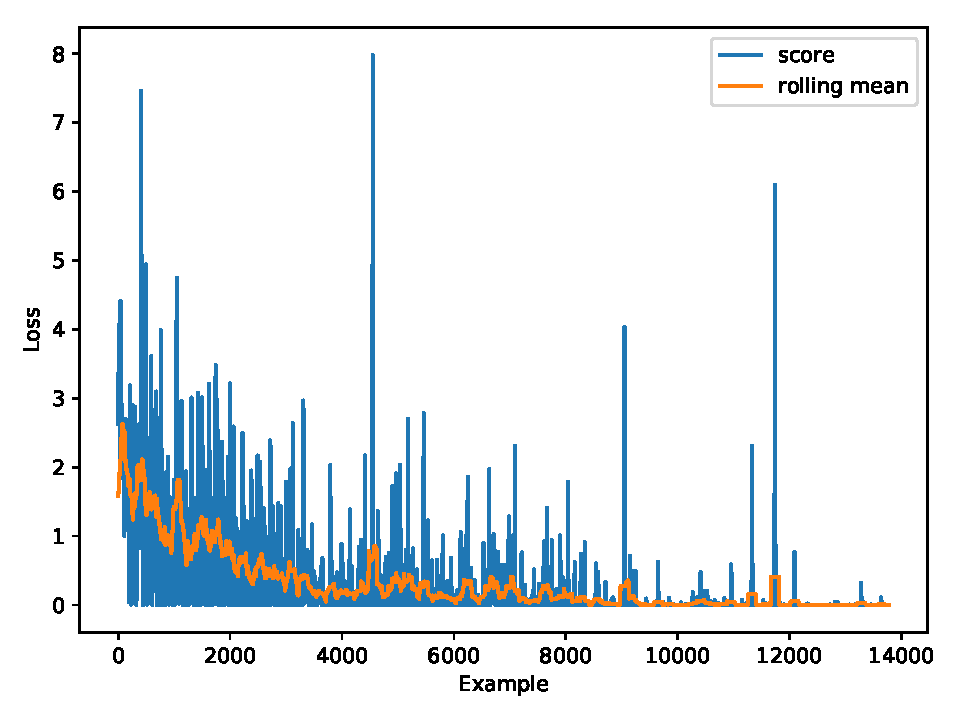
\includegraphics[width=.8\textwidth]{../figures/score_test}
  \caption{The learning curve of the dead wire fault classifier
    shows many rough spikes but eventually leads to convergence.}
  \label{fig:learning-curve}
\end{figure}

\subsection{Training Results}

The training performance of every single binary classifier was
evaluated on 10,000 new randomly generated
examples using the common evaluation metrics as described in section
\ref{sec:classification-evaluation}. An overview of the results is
presented in the following paragraphs.

\paragraph{Dead Wire Classifier:}
\begin{itemize}
  \item Accuracy: \ldots
  \item Precision: \ldots
  \item Recall: \ldots
  \item F-Measure: \ldots
\end{itemize}
The confusion matrix of the dead wire classifier can be found in Table
\ref{tbl:confusion-deadwire}.
\begin{table}[h]
  \centering
  \renewcommand\theadfont{\bfseries}
  \begin{tabular}{|c|c|c|}
    \hline
    & \thead{Dead Wire\\(Predicted)} & \thead{No Dead Wire\\(Predicted)} \\
    \hline
    \thead{Dead Wire\\(Actual)} & True Positives (TP) & False
    Negatives (FN) \\
    \hline
    \thead{No Dead Wire\\(Actual)} & False Positives (FP) & True
    Negatives (TN) \\
    \hline
  \end{tabular}
  \caption{Confusion matrix of the dead wire classifier.}
  \label{tbl:confusion-deadwire}
\end{table}

\paragraph{Dead Pin Classifier:}
\begin{itemize}
  \item Accuracy: 99.93\%
  \item Precision: 100.00\%
  \item Recall: 99.85\%
  \item F-Measure: 99.92\%
\end{itemize}
The confusion matrix of the dead pin classifier can be found in Table
\ref{tbl:confusion-pin}.
\begin{table}[h]
  \centering
  \renewcommand\theadfont{\bfseries}
  \begin{tabular}{|c|c|c|}
    \hline
    & \thead{Dead Pin\\(Predicted)} & \thead{No Dead Pin\\(Predicted)} \\
    \hline
    \thead{Dead Pin\\(Actual)} & 4799 & 7\\
    \hline
    \thead{No Dead Pin\\(Actual)} & 0 & 5194\\
    \hline
  \end{tabular}
  \caption{Confusion matrix of the dead pin classifier.}
  \label{tbl:confusion-pin}
\end{table}

\paragraph{Dead Connector Classifier:}
\begin{itemize}
  \item Accuracy: 98.43\%
  \item Precision: 98.37\%
  \item Recall: 95.21\%
  \item F-Measure: 96.79\%
\end{itemize}
The confusion matrix of the dead connector classifier can be found in
Table \ref{tbl:confusion-connector}.
\begin{table}[h]
  \centering
  \renewcommand\theadfont{\bfseries}
  \begin{tabular}{|c|c|c|}
    \hline
    & \thead{Dead Connector\\(Predicted)} & \thead{No Dead Connector\\(Predicted)} \\
    \hline
    \thead{Dead Connector\\(Actual)} & 2347 & 118 \\
    \hline
    \thead{No Dead Connector\\(Actual)} & 39 & 7496 \\
    \hline
  \end{tabular}
  \caption{Confusion matrix of the dead connector classifier.}
  \label{tbl:confusion-connector}
\end{table}

\paragraph{Dead Fuse Classifier:}
\begin{itemize}
  \item Accuracy: 99.02\%
  \item Precision: 98.61\%
  \item Recall: 97.18\%
  \item F-Measure: 97.89\%
\end{itemize}
The confusion matrix of the dead fuse classifier can be found in Table
\ref{tbl:confusion-fuse}.
\begin{table}[h]
  \centering
  \renewcommand\theadfont{\bfseries}
  \begin{tabular}{|c|c|c|}
    \hline
    & \thead{Dead Fuse\\(Predicted)} & \thead{No Dead Fuse\\(Predicted)} \\
    \hline
    \thead{Dead Fuse\\(Actual)} & 2272 & 66\\
    \hline
    \thead{No Dead Fuse\\(Actual)} & 32 & 7630\\
    \hline
  \end{tabular}
  \caption{Confusion matrix of the dead fuse classifier.}
  \label{tbl:confusion-fuse}
\end{table}

\paragraph{Dead Channel Classifier:}
\begin{itemize}
  \item Accuracy: 99.04\%
  \item Precision: 97.91\%
  \item Recall: 99.44\%
  \item F-Measure: 98.67\%
\end{itemize}
The confusion matrix of the dead channel classifier can be found in Table
\ref{tbl:confusion-channel}.
\begin{table}[h]
  \centering
  \renewcommand\theadfont{\bfseries}
  \begin{tabular}{|c|c|c|}
    \hline
    & \thead{Dead Channel\\(Predicted)} & \thead{No Dead Channel\\(Predicted)} \\
    \hline
    \thead{Dead Channel\\(Actual)} & 3552 & 20\\
    \hline
    \thead{No Dead Channel\\(Actual)} & 76 & 6352\\
    \hline
  \end{tabular}
  \caption{Confusion matrix of the dead channel classifier.}
  \label{tbl:confusion-channel}
\end{table}

\paragraph{Hot Wire Classifier:}
\begin{itemize}
  \item Accuracy: 100.00\%
  \item Precision: 100.00\%
  \item Recall: 100.00\%
  \item F-Measure: 100.00\%
\end{itemize}
The confusion matrix of the hot wire classifier can be found in Table
\ref{tbl:confusion-hotwire}.
\begin{table}[h]
  \centering
  \renewcommand\theadfont{\bfseries}
  \begin{tabular}{|c|c|c|}
    \hline
    & \thead{Hot Wire\\(Predicted)} & \thead{No Hot Wire\\(Predicted)} \\
    \hline
    \thead{Hot Wire\\(Actual)} & 5510 & 0\\
    \hline
    \thead{No Hot Wire\\(Actual)} & 0 & 4490\\
    \hline
  \end{tabular}
  \caption{Confusion matrix of the hot wire classifier.}
  \label{tbl:confusion-hotwire}
\end{table}

\section{Evaluation on Real Data}
